%%%%%%%%%%%%%%%%%%%%%%%%%%%%%%%%%%%%%%%%%%%%%%%%%%%%%%%%%%%%%%%%%%%%%%%%

%%% LaTeX Template for AAMAS-2025 (based on sample-sigconf.tex)
%%% Prepared by the AAMAS-2025 Program Chairs based on the version from AAMAS-2025. 

%%%%%%%%%%%%%%%%%%%%%%%%%%%%%%%%%%%%%%%%%%%%%%%%%%%%%%%%%%%%%%%%%%%%%%%%

%%% Start your document with the \documentclass command.


%%% == IMPORTANT ==
%%% Use the first variant below for the final paper (including auithor information).
%%% Use the second variant below to anonymize your submission (no authoir information shown).
%%% For further information on anonymity and double-blind reviewing, 
%%% please consult the call for paper information
%%% https://aamas2025.org/index.php/conference/calls/submission-instructions-main-technical-track/

%%%% For anonymized submission, use this
\documentclass[sigconf,nonacm]{aamas} 

%%%% For camera-ready, use this
%\documentclass[sigconf]{aamas} 


%%% Load required packages here (note that many are included already).

\usepackage{balance} % for balancing columns on the final page
\usepackage{tikz}
\usepackage{graphicx}
\usepackage{float}
\usepackage{dblfloatfix}
\usepackage{placeins}
\usepackage{afterpage}
\usepackage{algorithm}
\usepackage[noend]{algpseudocode}
\usepackage{amsmath}
%\usepackage{amssymb}
\usepackage{amsthm}

%\theoremstyle{plain}
\newtheorem{theorem}{Theorem}[section]
\newtheorem{observation}[theorem]{Observation}

%%%%%%%%%%%%%%%%%%%%%%%%%%%%%%%%%%%%%%%%%%%%%%%%%%%%%%%%%%%%%%%%%%%%%%%%

%%% AAMAS-2025 copyright block (do not change!)

\setcopyright{ifaamas}
\acmConference[AAMAS '25]{Proc.\@ of the 24th International Conference
on Autonomous Agents and Multiagent Systems (AAMAS 2025)}{May 19 -- 23, 2025}
{Detroit, Michigan, USA}{A.~El~Fallah~Seghrouchni, Y.~Vorobeychik, S.~Das, A.~Nowe (eds.)}
\copyrightyear{2025}
\acmYear{2025}
\acmDOI{}
\acmPrice{}
\acmISBN{}


%%%%%%%%%%%%%%%%%%%%%%%%%%%%%%%%%%%%%%%%%%%%%%%%%%%%%%%%%%%%%%%%%%%%%%%%

%%% == IMPORTANT ==
%%% Use this command to specify your EasyChair submission number.
%%% In anonymous mode, it will be printed on the first page.

\acmSubmissionID{<<EasyChair submission id>>}

%%% Use this command to specify the title of your paper.

\title[AAMAS-2025 Formatting Instructions]{Interval Selection with Binary Predictions}

%%% Provide names, affiliations, and email addresses for all authors.

\author{Christodoulos Karavasilis}
\affiliation{
  \institution{University of Toronto}
  \city{Toronto}
  \country{Canada}}
\email{ckar@cs.toronto.edu}


%%% Use this environment to specify a short abstract for your paper.

\begin{abstract}
Following a line of work that takes advantage of vast machine-learned data to enhance online algorithms with (possibly erroneous) information about future inputs, we consider predictions in the context of deterministic algorithms for the problem of selecting a maximum weight independent set of intervals arriving on the real line. We look at two weight functions, unit (constant) weights, and weights proportional to the interval's length. In the classical online model of irrevocable decisions, no algorithm can achieve constant competitiveness (Bachmann et al. \cite{bachmann2013online} for unit, Lipton and Tomkins \cite{lipton1994online} for proportional). In this setting, we show that a simple algorithm that is faithful to the predictions is optimal, and achieves an objective value of at least $OPT-\eta$, with $\eta$ being the total error in the predictions, both for unit, and proportional weights.

When revocable acceptances (a form of \textit{preemption}) are allowed, the optimal deterministic algorithm for unit weights is $2k$-competitive \cite{borodin2023any}, where $k$ is the number of different interval lengths. We give an algorithm with performance $OPT -\eta$ (and therefore $1$-consistent), that is also $(2k+1)$-robust. For proportional weights, Garay et al. \cite{garay1997efficient} give an optimal $(2\phi +1)$-competitive algorithm, where $\phi$ is the golden ratio. We present an algorithm with parameter $\lambda > 1$ that is $\frac{3\lambda}{\lambda -1}$-consistent, and $\frac{4\lambda^2 + 2\lambda}{\lambda -1}$-robust. Although these bounds are not tight, we show that for $\lambda > 3.42$ we achieve consistency better than the optimal online guarantee in \cite{garay1997efficient}, while maintaining bounded robustness.

 We conclude with some experimental results on real-world data that complement our theoretical findings, and show the benefit of prediction algorithms for online interval selection, even in the presence of high error.
\end{abstract}

%%% The code below was generated by the tool at http://dl.acm.org/ccs.cfm.
%%% Please replace this example with code appropriate for your own paper.


%%% Use this command to specify a few keywords describing your work.
%%% Keywords should be separated by commas.

\keywords{online algorithms, predictions, interval selection, scheduling}

%%%%%%%%%%%%%%%%%%%%%%%%%%%%%%%%%%%%%%%%%%%%%%%%%%%%%%%%%%%%%%%%%%%%%%%%

%%% Include any author-defined commands here.
         
\newcommand{\BibTeX}{\rm B\kern-.05em{\sc i\kern-.025em b}\kern-.08em\TeX}

%%%%%%%%%%%%%%%%%%%%%%%%%%%%%%%%%%%%%%%%%%%%%%%%%%%%%%%%%%%%%%%%%%%%%%%%

\begin{document}

%%% The following commands remove the headers in your paper. For final 
%%% papers, these will be inserted during the pagination process.

\pagestyle{fancy}
\fancyhead{}

%%% The next command prints the information defined in the preamble.

\maketitle 

%%%%%%%%%%%%%%%%%%%%%%%%%%%%%%%%%%%%%%%%%%%%%%%%%%%%%%%%%%%%%%%%%%%%%%%%

\section{Introduction}
\section{Introduction}
\label{sec:intro}

\begin{figure*}[tb]
    \centering
    \includegraphics[width=0.848\linewidth]{figs/circuitnn.pdf} 
    \caption{Illustration of differentiable CircuitNN. CircuitNN is designed based on differentiable NAND gates. After DAS is guided by PI and PO pairs of the truth table, CircuitNN can get the precise circuit architecture logic equivalent to the truth table.}
    \label{fig:circuitnn}
\end{figure*}

% 1. Describe the importance of logic synthesis
% 2. Existing Problems
% (a) Neural Architecture Search: Unstable, Predefined Setting, etc.
% (b) Circuit Generation: Probabilistic Model, Logic Equivalence

With the rapid advancement of technology, the scale of integrated circuits (ICs) has expanded exponentially. 
This expansion has introduced significant challenges in chip manufacturing, particularly concerning power and area metrics.
A primary objective in IC design is achieving the same circuit function with fewer transistors, thereby reducing power usage and area occupancy.

Logic synthesis~\cite{hachtel2005logicsynth}, a critical step in electronic design automation (EDA), transforms behavioral-level circuit designs into optimized gate-level circuits, ultimately yielding the final IC layout. 
The primary goal of logic synthesis is to identify the physical implementation with the fewest gates for a given circuit function. 
This task constitutes a challenging NP-hard combinatorial optimization problem. 
Current logic synthesis tools~\cite{brayton2010abc, wolf2013yosys} rely on human-designed heuristics, often leading to sub-optimal outcomes.

Differentiable architecture search (DAS) techniques~\cite{liu2018darts, chu2020darts} offer novel perspectives on addressing challenges in this problem.
Circuit functions can be represented through truth tables, which map binary inputs to their corresponding outputs. 
Truth tables provide a precise representation of input-output relationships, ensuring the design of functionally equivalent circuits.
Inspired by this, researchers~\cite{deepmind2024ai4sys, wang2024tnet} have begun exploring the application of DAS to synthesize circuits directly from truth tables.
Specifically, \citet{deepmind2024ai4sys} proposed CircuitNN, a framework that learns differentiable connection structures with logic gates, enabling the automatic generation of logic circuits from truth tables.
This approach significantly reduces the complexity of traditional circuit generation. 
Building on this, \citet{wang2024tnet} introduced T-Net, a triangle-shaped variant of CircuitNN, incorporating regularization techniques to enhance the efficiency of DAS.

Despite these advancements, several challenges remain. 
The computational complexity of DAS grows quadratically with the number of gates, posing scalability issues.
Although triangle-shaped architecture~\cite{wang2024tnet} partially mitigates this problem, redundancy persists. 
%Additionally, DAS is susceptible to converging to local optima, limiting the ability to search architectures that satisfy the given truth tables~\cite{liu2018darts}. 
%Furthermore, hyperparameters (network depth and layer width) require extensive searches, introducing complexity and prolonging the synthesis process. 
Additionally, DAS is susceptible to converging to local optima~\cite{liu2018darts} and hyperparameters (network depth and layer width) require extensive searches. 
The challenges arise from the vast search space in DAS. 
% Even with predefined settings for CircuitNN, finding a configuration that meets the truth table requires extensive trial and error during the DAS process. 
Intuitively, limiting the search space through predefined parameters (network depth, gates per layer, and connection probabilities) can significantly reduce the complexity.

Recent advances~\cite{openai2023gpt4, abramson2024alphafold3, esser2024sd3, li2024mar} in conditional generative models have demonstrated remarkable performance across language, vision, and graph generation tasks. 
Motivated by these developments, we propose a novel approach to circuit generation that generates preliminary circuit structures to guide DAS in generating refined circuits matching specified truth tables. 
Firstly, we introduce CircuitVQ, a tokenizer with a discrete codebook for circuit tokenization. 
Built upon our Circuit AutoEncoder framework~\cite{hou2022graphmae,li2023maskgae,wu2025mgvga}, CircuitVQ is trained through a circuit reconstruction task. 
Specifically, the CircuitVQ encoder encodes input circuits into discrete tokens using a learnable codebook, while the decoder reconstructs the circuit adjacency matrix based on these tokens.
Subsequently, the CircuitVQ encoder serves as a circuit tokenizer for CircuitAR pretraining, which employs a masked autoregressive modeling paradigm~\cite{chang2022maskgit, li2023mage}. 
In this process, the discrete codes function as supervision signals. 
After training, CircuitAR can generate discrete tokens progressively, which can be decoded into initial circuit structures by the decoder of the CircuitVQ. 
These prior insights can guide DAS in producing refined circuits that match the target truth tables precisely.

Our key contributions can be summarized as follows:
\begin{itemize}
\item We introduce CircuitVQ, a circuit tokenizer that facilitates graph autoregressive modeling for circuit generation, based on our Circuit AutoEncoder framework;
\item Develop CircuitAR, a model trained using masked autoregressive modeling, which generates initial circuit structures conditioned on given truth tables;
\item Propose a refinement framework that integrates differentiable architecture search to produce functionally equivalent circuits guided by target truth tables;
\item Comprehensive experiments demonstrating the scalability and capability emergence of our CircuitAR and the superior performance of the proposed circuit generation approach.
\end{itemize}

% Motivation
% (a) Diffusion (Vision, Graph), Autoregressive (Language, Vision)
% (b) Circuit Generation for Predefined Setting
% (c) Neural Architecture Search for Strict Logic Equivalence

% Contribution
% (a) Circuit Tokenizer (new transformer arch, training strategy)
% (b) CircuitAR (train and gen strategies, post-ar strategy)
% (c) Extensive Evaluation including BitD (Bit Distance) for Scalability


%%%%%%%%%%%%%%%%%%%%%%%%%%%%%%%%%%%%%%%%%%%%%%%%%%%%%%%%%%%%%%%%%%%%%%%%

\section{Problem Setting, Definitions and Discussion} \label{section:prelim}
\section{Preliminary}

\paragraph{Notation} Consider a sentence of $T$ tokens $\vx=\{\vx_1,\ldots, \vx_T\}\in\gX$, and let $P$ be the unknown target language distribution, $\tilde P(\vx)$ be the empirical distribution of the training data (which is an approximation of $P$), and $Q$ be the distribution of our model at hand. Since our paper is also closely related to RLHF, we will also use $\pi$ to represent the distributions. In particular, we sometimes write $\pi_\theta$ for a distribution that is parameterized by $\theta$, where $\theta$ is usually the set of trainable parameters of the LLM; we write $\pr$ for a reference distribution that should be clear given the context. The next token prediction loss is minimizing the forward-KL between $P$ and $Q$. 





%%%%%%%%%%%%%%%%%%%%%%%%%%%%%%%%%%%%%%%%%%%%%%%%%%%%%%%%%%%%%%%%%%%%%%%%

\section{Irrevocable Acceptances}\label{section:irrev}
In utilizing access to predictions, a natural algorithm to first consider is one that simply \textit{follows the predictions}. We therefore present algorithm \ref{alg:naive}, which is the main subject of this section.

\begin{algorithm}
\caption{\texttt{Naive}}\label{alg:naive}
\begin{algorithmic}
\State On the arrival of $I$:
\State $I_{s} \gets $ Set of intervals currently in the solution conflicting with $I$
\If{$Prd(I) = 1$ and $I_{s} = \emptyset$}
    \State Take $I$
\EndIf
\end{algorithmic}
\end{algorithm}
\textbf{Unit weights.} We first consider the case of unit weights, and prove the following (positive) result on the performance of algorithm \texttt{Naive}.




\begin{theorem}
    Algorithm Naive achieves $ALG \geq OPT - \eta$ for interval selection with unit weights.
    \label{theo:unw-naive-pos}
\end{theorem}
\begin{proof}
The proof works by mapping optimal intervals to error, and to intervals taken by the algorithm, given that every missed optimal interval can be associated with at least one unit of error. Let $OPT$ be an optimal solution, and let $ALG$ be the algorithm's solution. For each unit of error, we define an error element $h$.
Let $H=\{h_{1},...,h_{\eta}\}$ be the set of error elements. Let $H_{I} \subseteq H$, be the set of error elements corresponding to the error $\eta(I)$. It holds that $H_{I} \cap H_{J} = \emptyset$ for any two distinct intervals $I,J$, and $\bigcup\limits_{I} H_{I} = H$.\\\\
We define an injective mapping $F: OPT \rightarrow ALG \cup H$ as follows: Let $I_{opt}$ be an optimal interval. If $I_{opt}$ is taken by the algorithm, it is mapped onto itself. If $I_{opt}$ is not taken by the algorithm, there are two possibilities. The first possibility is that $Prd(I_{opt}) = 1$, but $I_{opt}$ conflicted with another interval $I_{c}$ taken by the algorithm. For $I_{c}$ to have been taken, it means that $Prd(I_{c}) = 1$, and $|H_{I_{c}} \cup \{I_c\}|>0$ because $I_c$ conflicts with $I_{opt}$. In this case we map $I_{opt}$ to an error element $h_{c}\in H_{I_{c}}$, or $I_c$ itself. Even if more optimal intervals were not taken because they conflicted with $I_{c}$, there will be enough distinct elements in $H_{I_{c}} \cup \{I_c\}$ to map them to.\\\\
The second possibility is that $I_{opt}$ was not taken, because $Prd(I_{opt}) = 0$. In this case, we have that $|H_{I_{opt}}| = 1$, and we can map $I_{opt}$ to the error element of its own prediction. In conclusion, we have that $ALG + |H| \geq OPT$, and we get the desired bound.    
\end{proof}
\begin{corollary}
Algorithm Naive is $1$-consistent.
\end{corollary}

\begin{theorem}
    For every deterministic algorithm, there exist a unit weights instance and predictions, such that $ALG = OPT - \eta$.
    \label{theo:unw-naive-neg}
\end{theorem}
\begin{proof}
    Let an interval $I_{big}$ arrive first, with $Prd(I_{big}) = 0$. If the algorithm rejects it, no more intervals arrive, and we have $ALG = 0$, $OPT = 1$, $\eta = 1$. If the algorithm takes $I_{big}$, two non-conflicting intervals arrive next, $I_{1}$ and $I_{2}$, both subsumed by $I_{big}$, with $Prd(I_{1}) = 0$ and $Prd(I_{2})=1$. In this case, we have $ALG = 1$, $OPT = 2$, $\eta = \eta(I_1) = 1$. In both cases, the equality holds. One can repeat this construction for an asymptotic result.
    \begin{figure}[h] % Adjust the width as needed
        \centering
        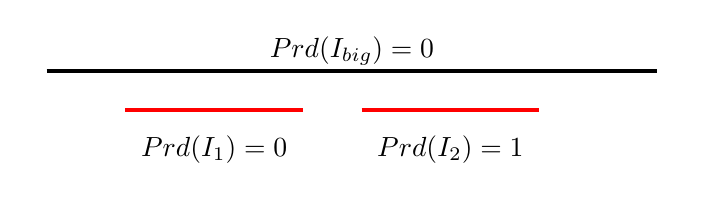
\begin{tikzpicture}[scale=0.5]
	
	\node at (0,0.5) {$Prd(I_{big}) = 0$};
	\node[draw=none] (I1a) at (-8,0) {$ $};
	\node[draw=none] (I1b) at (8,0) {$ $};
	\draw[line width=0.5mm] (I1a) -- (I1b);

	\node[draw=none] (I5a) at (-6,-1) {$ $};
	\node[draw=none] (I5b) at (-1,-1) {$ $};
	\node at (-3.5,-2) {$Prd(I_{1})=0$};
	\draw[color=red,line width=0.5mm] (I5a) -- (I5b);

 \node[draw=none] (I6a) at (0,-1) {$ $};
	\node[draw=none] (I6b) at (5,-1) {$ $};
	\node at (2.5,-2) {$Prd(I_{2})=1$};
	\draw[color=red,line width=0.5mm] (I6a) -- (I6b);

	\end{tikzpicture} 
        \caption{Instance of theorem \ref{theo:unw-naive-neg}.}
        \label{fig:neg-unit-irrev}
    \end{figure}
\end{proof}

\begin{corollary}
    Algorithm Naive is optimal for unit weights in the model of irrevocable acceptances.
\end{corollary}
Boyar et al. \cite{boyar2023online} were the first to consider the problem of interval selection with unit weights and irrevocable decisions, and they get the same (syntactically) performance, using a different algorithm, and a different set of predictions and error measure. In comparing our result to theirs, we note that our predictions are information theoretically strictly weaker than theirs\footnote{Their predictions consist of the entire input instance given in advance.}, and can in fact easily be extracted from theirs, allowing our algorithms to operate in their model. Furthermore, their predictions-following algorithm is enhanced with a \textit{greedy} aspect in order to achieve this optimal performance. As we will see in section \ref{section:exp}, experimental results on real-world data suggest that for some error ranges, pure \textit{greediness} is arguably a more important attribute than the use of predictions for getting a good solution, and the combination of both in the context of revocable acceptances works best.\\\\

We will now show that with \textbf{proportional weights}, algorithm \texttt{Naive} achieves the same performance bounds as in the case of unit weights.

\begin{theorem}
Algorithm Naive achieves $ALG \geq OPT - \eta$ for interval selection with proportional weights.
    \label{theo:prop-naive-pos}
\end{theorem}
\begin{proof}
        Without loss of generality, we assume integral lengths of intervals, and later explain how to generalize to real lengths. We discretize the weight of intervals into weight units, and define a weight element $w$ for each unit of weight. Let $W_{I} = \{w_{1},...,w_{w(I)}\}$ be the set of weight elements corresponding to the weight of interval $I$, with $W_{I} \cap W_{J} = \emptyset$ for any two distinct intervals $I,J$ . Let $W_{opt} = \bigcup_{I\in OPT}W_{I}$, and $W_{alg} = \bigcup_{I\in ALG}W_{I}$. The sets $H$ and $H_{I}$ are defined as for the unweighted algorithms. Lastly, let $C_{opt}(I)$ be the set of optimal intervals in $OPT$ that conflict with interval $I$.\\\\
    We argue for the existence of an injective mapping $F: W_{opt} \rightarrow W_{alg} \cup H$ as follows: Let $I_{opt}$ be an optimal interval. If $I_{opt}$ is taken by the algorithm, we map the elements of $W_{I_{opt}}$ to their corresponding elements in $W_{alg}$. If $I_{opt}$ is not taken by the algorithm, there are two cases. The first case is that $I_{opt}$ did not conflict with any interval in the solution, but $Prd(I_{opt}) = 0$. In this case, we know that $\eta(I_{opt}) = |H_{I_{opt}}| = w(I_{opt})$, and we can map the weight elements of $I_{opt}$ to error elements in $H_{I_{opt}}$.\\\\
    The other case is that $I_{opt}$ conflicted with at least one interval in the solution. Let that conflicting interval be $I_{c}$. It could also be that $Prd(I_{opt}) = 0$, and $H_{I_{opt}}$ would have error elements we can use, but we will assume the worst case of $Prd(I_{opt}) = 1$. In this case, it could be  $|W_{I_{opt}}| >  |H_{I_{c}}|$, and we cannot map the weight elements to error elements exclusively. We can, however, map the optimal weight elements, to elements in $H_{I_{c}} \cup W_{I_{c}}$. To see that there will always be sufficiently many unmapped elements, notice that $|H_{I_{c}} \cup W_{I_{c}}| \geq |\bigcup_{I \in C_{opt}(I_{c})}W_{I}|$. This is because $|H_{I_{c}}| = |\bigcup_{I \in C_{opt}(I_{c})}W_{I}| - |W_I|$, and $W_{I_c} \cap H_{I_c} = \emptyset$ always holds. We conclude that $|W_{alg}| + |H| \geq |W_{opt}|$, and we get the desired bound.\\\\
    To adapt the proof to real lengths, instead of considering sets of error and weight elements, we can define a transport plan using two transport matrices $H$ and $W$ of size $OPT\times ALG$. $H_{ij}$ (respectively $W_{ij}$) corresponds to the (real) amount of weight, or mass, mapped from $I_i \in OPT$ to the amount of error (resp. weight) introduced by $I_j \in ALG$. We can define these matrices such that for $1 \leq i \leq OPT$, $\sum_{1\leq j \leq ALG} H_{ij} + W_{ij} = w(I_i)$, for $1\leq j \leq ALG$, we have that $\sum_{1\leq i \leq OPT}H_{ij} \leq \eta(I_j)$ and $\sum_{1\leq i \leq OPT}W_{ij} \leq w(I_j)$.
\end{proof}
\begin{theorem}
For every deterministic algorithm, there exist a proportional weights instance and predictions, such that $ALG = OPT - \eta$.
    \label{theo:prop-naive-neg}
\end{theorem}
\begin{proof}
    Let $I_{1}$ arrive first with $Prd(I_{1}) = 0$. If the algorithm doesn't accept $I_{1}$, no more intervals arrive, and we have that $ALG = 0$, $OPT = w(I_{1})$, and $\eta = w(I_{1})$. If the algorithm accepts $I_{1}$, let two intervals $I_2$ and $I_3$ arrive next, with $w(I_2) = w(I_1)$, $Prd(I_2) = 1$, $w(I_3) = 2w(I_1)$ and $Prd(I_3) = 0$. In this case we have $ALG = w(I_1)$, $OPT = 3w(I_1)$, and $\eta = \eta(I_3) = 2w(I_1)$. In both cases the equality holds. One can repeat this construction for an asymptotic result.
\end{proof}

    \begin{figure}
	\centering
	
	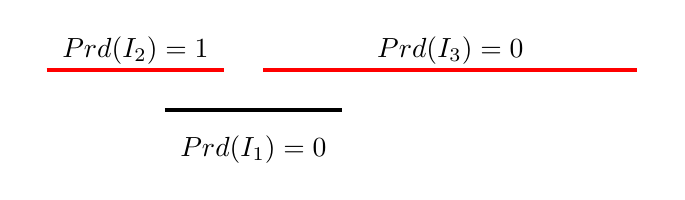
\begin{tikzpicture}[scale=0.5]

	\node at (-5,-2) {$Prd(I_{1}) = 0$};
	\node[draw=none] (I1a) at (-7.5,-1) {$ $};
	\node[draw=none] (I1b) at (-2.5,-1) {$ $};
	\draw[line width=0.5mm] (I1a) -- (I1b);
	
	
	%\node[draw=none] (d1) at (-3,-1) {$\rvdots$};

	
	\node[draw=none] (I3a) at (-10.5,0) {$ $};
	\node[draw=none] (I3b) at (-5.5,0) {$ $};
	\node at (-8,0.5) {$Prd(I_{2}) = 1$};
	\draw[color=red,line width=0.5mm] (I3a) -- (I3b);
	
	\node[draw=none] (I4a) at (-5,0) {$ $};
	\node[draw=none] (I4b) at (5,0) {$ $};
	\node at (0,0.5) {$Prd(I_{3}) = 0$};
	\draw[color=red,line width=0.5mm] (I4a) -- (I4b);

	\end{tikzpicture} 
	\caption{Instance of Theorem \ref{theo:prop-naive-neg}, with $w(I_2) = w(I_1), w(I_3) = 2w(I_1)$.}\label{fig:prop-neg-no-rev}
\end{figure}

\begin{corollary}
 Algorithm Naive is optimal for proportional weights in the model of irrevocable acceptances.
\end{corollary}
%%%%%%%%%%%%%%%%%%%%%%%%%%%%%%%%%%%%%%%%%%%%%%%%%%%%%%%%%%%%%%%%%%%%%%%%
\section{Revocable Acceptances}\label{section:rev}
Given the difficulty of the problem(s) in the conventional online model, we now consider the case where acceptances are revocable, but rejections are final, a relaxation of the model that is commonly studied for the problem of interval selection. A new interval can now always be accepted by displacing any intervals in the solution conflicting with it. For unit weights, Borodin and Karavasilis \cite{borodin2023any} give an optimal algorithm that is $2k$-competitive, where $k$ is the number of distinct interval lengths. We will refer to this algorithm of \cite{borodin2023any} as the \textit{BK2K} algorithm. \textit{BK2K} is a greedy algorithm, always accepting a new interval when there is no conflict, and whenever a conflict exists, the new interval is accepted only if it is properly included in an interval currently in the solution. We use that as the base logic for our predictions algorithm, and add one more replacement rule, which accepts a new interval $I$ that is only involved in partial conflicts, if $Prd(I) = 1$. Furthermore, an interval accepted by that rule gets marked, to make sure it cannot be replaced by that rule again. We call this algorithm \texttt{Revoke-Unit} \ref{alg:unw-revoke}. Interestingly, this rule of locally \textit{following the predictions once}, suffices to give us $1$-consistency.




\begin{algorithm}
\caption{\texttt{Revoke-Unit}}\label{alg:unw-revoke}
\begin{algorithmic}
\State $M \gets \emptyset$ \Comment{Set of marked intervals}
\State $S \gets \emptyset$ \Comment{Solution set}
\State On the arrival of $I$:
\State $I_{s} \gets $ Set of intervals currently in the solution conflicting with $I$
\If{$I_{s} = \emptyset$ or ($I_{s}=\{I'\}$ and $I \subset I'$)}
    \If{ $I' \in M$}
        \State $M \gets M \cup \{I\}$
    \EndIf
    \State $S \gets S \cup \{I\} \setminus \{I'\} $\Comment{Take $I$ and discard $I'$ if necessary}
\ElsIf{$I$ is only involved in partial conflicts \textbf{and} $Prd(I) = 1$ \textbf{and} $I_{s} \cap M = \emptyset$}
    \State $S \gets S \cup \{I\} \setminus I_s $\Comment{Take $I$ and discard conflicting intervals}
    \State $M \gets M \cup \{I\}$
\EndIf
\end{algorithmic}
\end{algorithm}
%Algorithm \ref{alg:unw-revoke} is a greedy algorithm that uses the same replacement rule (replace when new interval entirely subsumed by existing one) as the optimal $2k$ online algorithm, but has one additional replacement rule for partial conflicts. If the newly arrived interval is only involved in partial conflicts (can only be one or two such conflicts at most), the prediction says it's optimal, and the existing intervals it conflicts with are unmarked (have not been involved in a partial-conflict replacement in the past), then it accepts the new interval. {\color{red} Talk about how follow-the-prediction-ONCE works is the main idea, and suffices for 1-consistency. Also mention the BK2K notation.}

\begin{theorem}
    Algorithm \ref{alg:unw-revoke} achieves $ALG \geq OPT - \eta$.
\end{theorem}
\begin{proof}
    We follow the same approach as in the proof of Theorem \ref{theo:unw-naive-pos}, mapping optimal intervals to intervals taken by the algorithm, and to error. The main difference is that because of revoking, this mapping might be redefined throughout the execution of the algorithm. As before, we let $H$ be the set of error elements, and $H_{I} \subseteq H$ be the set of error elements introduced by $\eta(I)$. Let $I_{opt}$ be an optimal interval. We will define an injective mapping $F: OPT \rightarrow ALG \cup H$ as follows: If $I_{opt}$ is taken by the algorithm, it is initially mapped onto itself. If $I_{opt}$ is later replaced, it must be because of a partial conflict (w.l.o.g. no interval is subsumed by an optimal interval) with a new interval $I'$ with $Prd(I') = 1$. In this case, $I_{opt}$ will be mapped to an error element in $H_{I'}$, or if no further optimal intervals that conflict with $I$ are yet to arrive, it will be mapped to $I$. In both, subcases it will never be remapped.\\
    Consider now the case of $I_{opt}$ being rejected upon arrival. This can only happen if it is involved in (at most two) partial conflicts. There are two possible cases. The first case is that $Prd(I_{opt}) = 0$, and therefore $|H_{I_{opt}}| = 1$, in which case we map $I_{opt}$ to the error element of its own prediction. The second case is that $Prd(I_{opt}) = 1$, but at least one of the conflicting intervals was marked. Let $I_{c}$ be one of the marked, partially conflicting intervals. If $I_{c}$ was marked by being taken through a partial-conflict replacement, it means that $Prd(I_{c}) = 1$, and $|H_{I_{c}} \cup \{I_c\}| > 0$, in which case we can map $I_{opt}$ to an element $h_{c} \in H_{I_{c}}\cup \{I_c\}$.\\
    If $I_{c}$ was instead marked by a proper-inclusion-replacement, we trace the original interval that got marked through a partial-conflict-replacement. Call that interval $I^{'}_{c}$. It holds that $I^{'}_{c}$ conflicts with $I_{c}$, and therefore also conflicts with $I_{opt}$. Moreover, for $I^{'}_{c}$ to have been accepted, it must be that $Prd(I^{'}_{c})=1$ and $|H_{I^{'}_{c}} \cup \{I^{'}_{c}\}|>0$. In this case, we map $I_{opt}$ to an element $h_{c'} \in H_{I^{'}_{c}} \cup \{I^{'}_{c}\}$. In conclusion, we have that $ALG + |H| \geq OPT$, and we get the desired bound.
\end{proof}

We note that the performance of algorithm \ref{alg:unw-revoke} on the instance of Theorem \ref{theo:unw-naive-neg} is exactly equal to $OPT - \eta$, and we get the following lemma.

\begin{lemma}
    The performance of algorithm \ref{alg:unw-revoke} cannot be better than $OPT-\eta$.
\end{lemma}

We next show that the robustness of algorithm \texttt{Revoke-Unit} nearly matches the optimal online guarantee.

\begin{theorem} \label{theo:unw-rev-robust}
    With at most $k$ distinct interval lengths, algorithm \ref{alg:unw-revoke} is $(2k+1)$-robust.
\end{theorem}
\begin{proof}
    We use a charging argument and show that an interval taken by the algorithm can be charged by at most $2k+1$ optimal intervals. As soon as an optimal interval arrives, we map it to an interval already taken by the algorithm or itself. When an interval is replaced during the execution, all optimal intervals charged to it up to that point, will now be charged to the new interval that was accepted. We build upon the proof of Theorem 3.2 in \cite{borodin2023any}. In the case of the \textit{BK2K} algorithm (\cite{borodin2023any}), it is true that for every predecessor trace $\mathcal{P}$, and consecutive intervals $(I_i,I_{i+1}) \in \mathcal{P}$, $\Phi(I_{i+1}) \leq \Phi(I_i) + 2$, and the length of every predecessor trace is at most $k$. While the former is still true for algorithm \texttt{Revoke-Unit}, the latter is not, and that is because we have an additional replacement rule. However, we argue that for every $I_i \in \mathcal{P}$, if $I_j,\; j > i$ is the next interval in the trace that was accepted through proper-inclusion, it is true that $TC(I_j) \leq TC(I_i) + 3$.\\
    
    Figure \ref{fig:pcr-charge} shows how to maximize charge on the event of a partial-conflict replacement. Before being replaced by a partially-conflicting interval, $I_{1}$ can be directly charged by at most two optimal intervals ($I^{1}_{opt}, I^{2}_{opt}$), one on each side. After $I_{2}$ replaces $I_{1}$, it can also be directly charged by two optimal intervals, but only if $I^{2}_{opt}$ was not charged to $I_{1}$ earlier. In other words, if $I_{2}$ is directly charged by two new intervals, it means that $I_{1}$ was directly charged by at most one, concluding that $\Phi(I_2) \leq TC(I_1) + 3$.

    \begin{figure}[H]
	\centering
	
	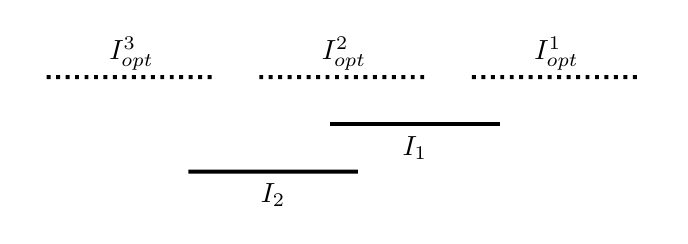
\begin{tikzpicture}[scale=0.6]

	\node at (-5,-1.5) {$I_{2}$};
	\node[draw=none] (I1a) at (-7,-1) {$ $};
	\node[draw=none] (I1b) at (-3,-1) {$ $};
	\draw[line width=0.5mm] (I1a) -- (I1b);
	
	
	%\node[draw=none] (d1) at (-3,-1) {$\rvdots$};

	\node[draw=none] (I2a) at (-5.5,1) {$ $};
	\node[draw=none] (I2b) at (-1.5,1) {$ $};
	\node at (-3.5,1.5) {$I^{2}_{opt}$};
	\draw[dotted,line width=0.5mm] (I2a) -- (I2b);
	
	\node[draw=none] (I3a) at (-10,1) {$ $};
	\node[draw=none] (I3b) at (-6,1) {$ $};
	\node at (-8,1.5) {$I^{3}_{opt}$};
	\draw[dotted,line width=0.5mm] (I3a) -- (I3b);
	
	\node[draw=none] (I4a) at (-4,0) {$ $};
	\node[draw=none] (I4b) at (0,0) {$ $};
	\node at (-2,-0.5) {$I_{1}$};
	\draw[line width=0.5mm] (I4a) -- (I4b);
	
	\node[draw=none] (I5a) at (-1,1) {$ $};
	\node[draw=none] (I5b) at (3,1) {$ $};
	\node at (1,1.5) {$I^{1}_{opt}$};
	\draw[dotted,line width=0.5mm] (I5a) -- (I5b);

	\end{tikzpicture} 
	\caption{Maximum charge through partial-conflict replacement.}\label{fig:pcr-charge}
\end{figure}

Finally, notice that because the mark of an interval carries over when it is replaced, the event of a partial-conflict replacement can occur at most once in each predecessor trace,
and excluding at most one subsequence $(I_i, I_r, I_j) \in \mathcal{P}$ where $TC(I_j) \leq TC(I_i) + 3$, it holds that for $(I_b,I_{b+1}) \in \mathcal{P}$, $\Phi(I_{b+1})\leq \Phi(I_b) + 2$, giving us a worst case competitive ratio of $2k+1$. 
\end{proof}

\begin{corollary}
    With at most $k$ distinct interval lengths, and predictions with total error $\eta$, Algorithm Revoke-Unit achieves $ALG \geq \max\{OPT-\eta , \frac{OPT}{2k+1}\}$.
\end{corollary}

Notice how we can choose not to carry over the mark when proper-inclusion replacement occurs, and get a $3k$-robust algorithm. Such an algorithm is prone to follow the prediction more often, and it can outperform \texttt{Revoke-Unit} for some small values of error caused by adversarial predictions.\\\\
We now look at the case of proportional weights. In the conventional online setting, Garay et al. \cite{garay1997efficient} give a $2\phi + 1  \approx 4.236-$competitive algorithm, while Tomkins \cite{tomkins1995lower} gives a matching lower bound. They call their optimal algorithm \texttt{LR} (for \textit{length of route}), and we include it here for completeness. Unlike the case of unit weights, we now want to accept intervals that occupy as much of the line as possible. Algorithm \texttt{LR} works greedily by always accepting a new interval with no conflicts, and when there are conflicts, it accepts the new interval if its length is at least $\phi$ times greater than the largest conflicting interval. More generally, using parameter $\beta \geq \phi$, we have the following lemma:
\begin{lemma}[Garay et al. \cite{garay1997efficient}]
    Algorithm \texttt{LR} with parameter $\beta \geq \phi$ is $(2\beta + 1)$-competitive for the problem of interval selection with proportional weights.
\end{lemma}
\begin{algorithm}
\caption{LR \cite{garay1997efficient}}\label{alg:garay_prop}
\begin{algorithmic}
\State Parameter $\beta = \phi$ \Comment{optimal value for parameter $\beta$}
\State On the arrival of $I$:
\State $I_{s} \gets $ Set of intervals currently in the solution conflicting with $I$
\If{ $w(I) > \beta \cdot \max\{w(J)\; : \; J\in I_s\}$}
    \State Accept $I$ and displace conflicts
    \State Return
\EndIf
\end{algorithmic}
\end{algorithm}
Instead of using algorithm \texttt{LR} as the base of our predictions algorithm, we consider a slightly modified version, which we refer to as \texttt{LR$'$}, and which compares the weight of the new interval to the sum of the weights of the conflicting intervals, instead of looking only at the longest interval. Although we do not know the exact performance of algorithm \texttt{LR$'$} in the online model, we conjecture it is also $(2\phi + 1)$-competitive.\\\\
In trying to utilize predictions in the case of proportional weights, we first make the following observations:
\begin{observation}
    $1$-consistency is unattainable while maintaining bounded robustness.
\end{observation}
\begin{proof}
    To be $1$-consistent, the algorithm must be able to replace an interval with an arbitrarily smaller one that is part of the optimal solution. The adversary could then stop the instance, forcing arbitrarily bad robustness.
\end{proof}

\begin{observation}
    In order to have bounded robustness, it must be that a new interval that is sufficiently large (small\footnote{More accurately, an interval reducing ALG sufficiently much. }) must always be accepted (rejected).
\end{observation}

\begin{definition}[$\alpha-$increasing]
    An $\alpha$-increasing algorithm never accepts a new conflicting interval
that is less than $\alpha$ times the longest interval it conflicts with.
\end{definition}
\begin{lemma}
    An $\alpha$-increasing algorithm (greedy or non-greedy), cannot be better than $(2\alpha +1)$-consistent.
\end{lemma}
\begin{proof}
    Let an interval $I_1$ arrive first. Let $I_2$ and $I_3$ be intervals that partially conflict with $I_1$ on either side, and $w(I_2) = w(I_3) = \alpha \cdot w(I_1) - \epsilon$. Let $I_4$ with $w(I_4) = w(I_1)-2\epsilon$ be an interval that is fully subsumed by $I_4$. This instance is depicted in figure \ref{fig:neg-alpha-increasing}. The algorithm will never replace $I_1$, while the optimal solution is made of $\{I_2,I_3,I_4\}$.
    \begin{figure}[h] % Adjust the width as needed
        \centering
        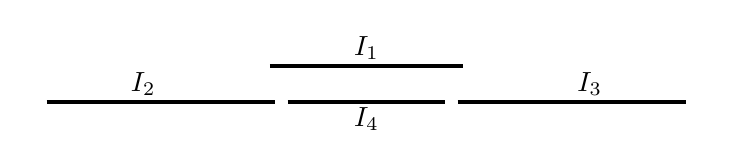
\begin{tikzpicture}[scale=0.45]
	
	\node at (0,0.5) {$I_1$};
	\node[draw=none] (I1a) at (-3,0) {$ $};
	\node[draw=none] (I1b) at (3,0) {$ $};
	\draw[line width=0.5mm] (I1a) -- (I1b);

 \node at (-6.3,-0.5) {$I_2$};
	\node[draw=none] (I2a) at (-9.3,-1) {$ $};
	\node[draw=none] (I2b) at (-2.3,-1) {$ $};
	\draw[line width=0.5mm] (I2a) -- (I2b);

  \node at (6.3,-0.5) {$I_3$};
	\node[draw=none] (I2a) at (2.3,-1) {$ $};
	\node[draw=none] (I2b) at (9.3,-1) {$ $};
	\draw[line width=0.5mm] (I2a) -- (I2b);

	\node[draw=none] (I5a) at (-2.5,-1) {$ $};
	\node[draw=none] (I5b) at (2.5,-1) {$ $};
	\node at (0,-1.5) {$I_{4}$};
	\draw[line width=0.5mm] (I5a) -- (I5b);

	\end{tikzpicture} 
        \caption{Consistency bound for $\alpha$-increasing algorithms.}
        \label{fig:neg-alpha-increasing}
    \end{figure}
\end{proof}
Algorithm \texttt{LR} is a $\phi$-increasing algorithm, while the algorithm by Woeginger \cite{woeginger1994line} for the real-time model is $2$-increasing. Our predictions algorithm \ref{alg:prop-revoke2} \texttt{Revoke-Proportional} is $1$-increasing. The algorithm works like \texttt{LR$'$}, with one additional replacement rule that accepts a new interval that is predicted to be optimal, even if it is not sufficiently larger than what it conflicts with. More precisely, if a new interval is predicted to be optimal and is at least as big as the sum of the weights of the intervals it conflicts with, and none of the conflicting intervals were predicted to be optimal, it will be accepted through the predictions rule. The algorithm takes a parameter $\lambda > 1$, which can be thought of as an indicator of how much the predictions are trusted. As $\lambda$ increases, the consistency bound improves.

\begin{algorithm}
\caption{\texttt{Revoke-Proportional} {\hfil Parameter: $\lambda > 1$ }}\label{alg:prop-revoke2}
\begin{algorithmic}
\State On the arrival of $I$:
\State $I_{s} \gets $ Set of intervals currently in the solution conflicting with $I$
\State Let $w_c = \sum_{J \in I_s} w(J)$ \Comment{Total weight of conflicting intervals}
\If{ $w(I) \geq \lambda\cdot w_c$} \Comment{Main replacement rule}
    \State Accept $I$ and displace conflicts
    \State Return
\ElsIf{$Prd(I) = 1$} \Comment{Predictions rule} 
    \If{($w(I) \geq w_c$ and $|\{J: J \in I_s \text{ and }Prd(J)=1\}| = \emptyset$)} 
    \State Accept $I$ and displace conflicts
    \State Return
    \EndIf
\EndIf
\end{algorithmic}
\end{algorithm}

\begin{theorem}
    Algorithm Revoke-Proportional is $\frac{3\lambda}{\lambda -1}$-consistent.\label{theo:prop-consistent}
\end{theorem}
\begin{proof}
We consider the optimal solution $OPT$ consistent with the fully accurate predictions. We will show that throughout the execution of the algorithm, we have that $\Phi(I) \leq \mu \cdot w(I)$, for every $I$ in the current solution. In the end, we have that $\sum_{I\in ALG} \Phi(I) = OPT$, giving us the $\mu$-consistency of the algorithm.\\\\
As in the proof of Theorem \ref{theo:unw-rev-robust}, we consider the notions of \textit{transfer charge} ($TC$), and \textit{direct charge} ($DC$). We can express $\Phi(I) = TC(I) + DC(I)$. A transfer charge occurs whenever accepting a new interval $I$ replaces intervals currently in the solution. In that case, the total charge of those conflicting intervals is passed on as transfer charge to $I$. Any additional charge to $I$ after its acceptance is through direct charge, namely rejection of subsequent optimal intervals conflicting with $I$. We will write $DC_J(I)$ to denote the amount of direct charge from interval $J$ to interval $I$. Whenever an optimal interval is accepted, we consider its weight being directly charged to itself, and it cannot be directly charged again.\\\\
Whenever an optimal interval is rejected upon arrival, we charge its weight to the intervals it conflicts with, with its weight being distributed to all its conflicting intervals, in proportion to their weight. Specifically, let $I_o$ be the newly arrived optimal interval that is rejected, and $I_s$ denote the set of conflicting intervals. Each interval $J \in I_s$ is directly charged $DC_{I_o}(J)=w(I_o) \frac{w(J)}{w_c}\leq w(I_o)$. Furthermore, for an optimal interval to have been rejected, it must be that even the predictions rule failed, and because the predictions are accurate, it must have failed because $w(I_o) < w_c$. Because of this, we get that $w(I_o) \frac{w(J)}{w_c} \leq w(J)$, and therefore $DC_{I_o}(J)\leq\min\{w(I_o),w(J)\}$. An interval $I \in ALG$ can be directly charged by at most three different types of optimal intervals: 1) smaller intervals that are subsumed by it, 2) an optimal interval partially conflicting on the left, and 3) an optimal interval partially conflicting on the right.
In the case of smaller optimal intervals subsumed by $I$, the total amount of direct charge from those intervals can be at most $w(I)$. Given that each of the two possible partially conflicting intervals can directly charge $I$ at most $w(I)$, we conclude that for every $I\in ALG$:
\begin{equation}
\label{dc-bound}
    DC(I) \leq 3w(I)
\end{equation}
We omitted the case where the rejected optimal interval subsumes $I$, because in that case $DC(I) = w(I)$ and \ref{dc-bound} holds trivially. We now focus on the total amount of charge on any interval $I\in ALG$. Let:
$$\mu = \frac{3\lambda}{\lambda - 1}$$
We want to make sure that throughout the execution of the algorithm, $\Phi(I) \leq \mu \cdot w(I)$. Before any interval is accepted through replacement, intervals in the solution could have only been directly charged through rejected optimal intervals, and because of \eqref{dc-bound}, and the fact that $\lambda > 1$, our desired bound holds. We now consider all the cases of an interval being accepted through replacement.\\\\
\underline{Case $1$}: $I$ is an optimal interval and it is accepted through the predictions rule. In this case we have that $DC(I) = w(I)$, and we need to look at $TC(I)$. Let $L_c$ and $R_c$ denote the intervals (if any) that $I$ is partially conflicting with on the left and on the right respectively, and let $M_c$ denote the set of intervals that $I$ subsumes. We know that all of these conflicting intervals are not optimal, and they were accepted through the algorithm's main rule. First, notice that for all $J\in M_c$, $DC(J) = 0$, and $\Phi(J) = TC(J) \leq \frac{\mu}{\lambda} \cdot w(J)$. Moreover, $L_c$ and $R_c$ had not yet been directly charged by a partially conflicting optimal interval on one side, and therefore we have that $\Phi(L_c) \leq \frac{\mu}{\lambda}\cdot w(L_c) + 2w(L_c)$, and similarly $\Phi(R_c) \leq \frac{\mu}{\lambda}\cdot w(R_c) + 2w(R_c)$.\\
Putting everything together:
\[
\begin{aligned}
    TC(I) &= \sum_{J\in M_c} \Phi(J) + \Phi(L_c) + \Phi(R_c) \\
     & \leq \frac{\mu}{\lambda}\cdot w_c + 2(w(L_c) + w(R_c))\\
     & \leq \left(\frac{\mu}{\lambda} + 2\right)w_c\\
     &\leq \left(\frac{\mu}{\lambda} + 2\right)w(I)
\end{aligned}
\]
The last inequality being true from the fact that the main predictions rule is satisfied. Given also that $DC(I) = w(I)$, we get that $\Phi(I) \leq (\frac{\mu}{\lambda} + 2)w(I) + w(I) = (\frac{\mu}{\lambda} + 3)w(I)$. With our choice of $\mu$, we have:
\[\begin{aligned}
    \Phi(I) &\leq \left(\frac{\frac{3\lambda}{\lambda - 1}}{\lambda} + 3 \right)w(I) \\
    &= \left(\frac{3\lambda}{\lambda -1}\right)w(I)\\\\
\end{aligned}\]
\underline{Case $2$}: $I$ is an optimal interval and it is accepted through the algorithm's main rule. This is similar to case 1, with $DC(I) = w(I)$ and $w(I)\geq \lambda \cdot w_c$. The same analysis gives us $TC(I)\leq \left( \frac{\mu}{\lambda} + 2 \right)\frac{w(I)}{\lambda}$, and because $\lambda > 1$, the same bound holds.\\\\
\underline{Case $3$}: $I$ is not an optimal interval and it is accepted through the algorithm's main rule. In this case we have that $DC(I) \leq 3w(I)$, and we get that
\[\begin{aligned}
    \Phi(I) & \leq \sum_{J\in I_s} \Phi(J) + 3w(I)\\
    & \leq \frac{\mu}{\lambda}\cdot w(I) + 3w(I)\\
    & = \left(\frac{3\lambda}{\lambda -1}\right)w(I)
\end{aligned}\]
In conclusion, we have that throughout the execution of the algorithm, for $I \in ALG$, $\Phi(I)\leq \frac{3\lambda}{\lambda - 1}w(I)$, and therefore $\frac{OPT}{ALG} \leq \frac{3\lambda}{\lambda - 1}$. 
\end{proof}
\vspace{0.5cm}
We see that as $\lambda \rightarrow \infty$, the algorithm's consistency goes to $3$. We now look at the robustness of algorithm \texttt{Revoke-Proportional}.\\
\begin{theorem}
    Algorithm Revoke-Proportional is $\frac{4\lambda^2 + 2\lambda}{\lambda -1}$-robust.
\end{theorem}
\begin{proof}
    The argument is similar to the proof of Theorem \ref{theo:prop-consistent}. Both \textit{direct}, and \textit{transfer} charging work the same way as before. Let $\mu = \frac{2\lambda^2 +3\lambda + 1}{\lambda -1 }$, and $\delta = 2\lambda + 1$. We will show that that for every $I \in ALG$, $\Phi(I)\leq (\mu + \delta)\cdot w(I)=\frac{4\lambda^2 + 2\lambda}{\lambda -1}w(I)$.\\\\
    Notice first that the upper bound on direct charging is not as good as before. More precisely, with $I_o$ being a newly arrived optimal interval that will be rejected and $I_s$ being its conflicting intervals currently in the solution, we have that for every $J\in I_s$, $DC_{I_o}(J)= w(I_o)\frac{w(J)}{w_c}\leq \lambda \cdot w(J)$. More generally, $DC_{I_o}(J) \leq \min\{w(I_o),\lambda\cdot w(J)\}$. As before, given the three different possible types of conflicts, we have that:
    \begin{equation}
        DC(I) \leq (2\lambda + 1)w(I)
    \end{equation}
    We can now bound the total amount of charge on every interval in the algorithm's solution, throughout its execution. Before any replacement happens, the bound $\Phi(I) \leq (\mu + \delta)\cdot w(I)$ holds trivially.\\\\
    \underline{Case $1$}: Interval $I$ is accepted through the algorithm's main rule. We get that:
    \[\begin{aligned}
        \Phi(I) &\leq (\mu + \delta)\cdot w_c + (2\lambda + 1)\cdot w(I)\\
        & \leq (\mu + \delta)\cdot \frac{w(I)}{\lambda} + (2\lambda + 1)\cdot w(I)\\
        & = \left(\frac{\mu + \delta}{\lambda} + 2\lambda + 1\right)w(I)\\
        & = \left( \frac{\frac{4\lambda^2 +2\lambda}{\lambda-1}+2\lambda^2 + \lambda}{\lambda} \right)w(I)\\
        & = \mu \cdot w(I)
    \end{aligned}\]
\underline{Case $2$}: Interval $I$ is accepted through the algorithm's predictions rule. Notice that in this case, all conflicting intervals must have been accepted through the main rule, and not the predictions rule. Because of this, as we showed in case $1$, for every $J\in I_s$, it holds that $\Phi(J) \leq \mu\cdot w(J)$. This helps us bound the amount of transfer charge to interval $I$.
\[\begin{aligned}
    \Phi(I) &\leq \mu \cdot w_c + (2\lambda + 1)\cdot w(I)\\
    & \leq \mu \cdot w(I) + (2\lambda + 1)\cdot w(I) \\
    & = (\mu + \delta)\cdot w(I)
\end{aligned}\]
To summarize, we have shown that in the worst case, $\Phi(I) \leq (\mu + \delta)\cdot w(I)$ for every $I\in ALG$. This concludes the proof.
\end{proof}

\begin{figure*}[t!]
\centering
\caption{\texttt{NASA-iPSC} dataset.} (a) Unit \& Irrevocable, (b) Unit \& Revoking, (c) Proportional \& Irrevocable, (d) Proportional \& Revoking
\includegraphics[width=\textwidth]{exp_pics/nasa/nasa_combined_ann.png}
\label{fig:nasa_exps}
\end{figure*}
\begin{figure*}[t!]
\centering
\caption{\texttt{CTC-SP2} dataset.}
\includegraphics[width=\textwidth]{exp_pics/ctc/ctc_combined_ann.png}
\label{fig:ctc_exps}
\end{figure*}

We note that for $\lambda > \frac{2+\sqrt{5}}{\sqrt{5} -1}\approx 3.42 $, the consistency of our algorithm is already better than $2\phi + 1$, and $22.15$-robust. We have shown we can get consistency better than the online bound of \texttt{LR}, while maintaining bounded robustness. We believe further improvement on the bounds of \texttt{Revoke-Proportional} is possible, with an analysis that looks more closely at the dependence between direct and transfer charging.\\
One may also be able to further improve the algorithm by accepting an interval that is not as big as the sum of its conflicts, making the algorithm $a$-increasing with $a<1$. This would relax the predictions rule further, and make the algorithm more prone to bad choices caused by misleading predictions. In our experiments, we briefly discuss one such algorithm, which we call \texttt{Revoke-Prop-Half}, and which can accept a supposedly optimal interval even if it is half as big as its conflicts.







%%%%%%%%%%%%%%%%%%%%%%%%%%%%%%%%%%%%%%%%%%%%%%%%%%%%%%%%%%%%%%%%%%%%%%%%

\section{Experimental Results}\label{section:exp}
\section{Experiments: Planning outperforms Heuristics}
\label{sec:experiment}

We begin our empirical demonstrations by showcasing the effectiveness of our planning framework on both synthetic and real datasets. We focus on the simplest planning algorithm, 1-step lookaheads (Algorithm~\ref{alg:complete}), and show that even basic planning can hold great promise. 
We illustrate our framework using two uncertainty quantification modules---GPs and 
\ensembles/ \ensembleplus. 

Throughout this section, we focus on evaluating the mean squared error of 
a regression model $\model$,  and develop adaptive policies that minimize uncertainty on $g(f)$ defined in~\eqref{eqn:l2-g-f}.
When GPs provide a valid model of uncertainty, 
our experiments show that our planning framework significantly outperforms other baselines. 
We further demonstrate that our conceptual framework extends to deep learning-based uncertainty quantification methods such as  \ensembleplus while highlighting computational challenges that need to be resolved in order to scale our ideas. 
For simplicity, we assume a naive predictor, i.e., $\psi(\cdot) \equiv 0$. However, we emphasize that this problem is just as complex as if we were using a sophisticated model $\psi(.)$. The performance gap between the algorithms 
primarily depends
on the level  of uncertainty in our prior beliefs.

To evaluate the performance of our algorithm, we benchmark it against several baselines. 
%Active learning baselines use an acquisition function $\ac$ to select points that have the highest   function value: $X\opt_t \in \argmax_{X \in \xpoolj{t}} \ac({X})$ at every step $t$. These methods may also need an UQ module, which we simply use the same UQ module as in our algorithm, and it  outputs $V(X)$ that measures the the uncertainty of each point $X \in \xpoolj{t}$.
Our first set of baselines are from active learning~\citep{AggarwalKoGuHaPh14}:
\\ % \noindent\textbf{Active Learning Heuristics:} 
\textbf{(1)} 
\textsf{Uncertainty Sampling (Static):}  In this approach, we query the samples for which the model is least certain about. Specifically, we estimate the variance of the latent output $f(X)$ for each $X \in \xpool$ using the UQ module and select the top-$K$ points with the highest uncertainty. \\
\textbf{(2)} \textsf{Uncertainty Sampling (Sequential):} This is a greedy heuristic that sequentially selects the points with the highest uncertainty within a batch, while updating the posterior beliefs using pseudo labels from the current posterior state. Unlike \textsf{Uncertainty Sampling (Static)}, this method takes into account the information gained from each point within batch, and hence tries to diversify the selected points within a batch. 

 
We also compare our approach to the  \textbf{(3)} \textsf{Random Sampling}, which selects each batch uniformly at random from the pool. Additionally, we compare solving the planning problem using  \textsf{REINFORCE}-based policy gradients with   $\mathsf{Smoothed\text{-}Autodiff}$ policy gradients.\footnote{Our code repository is available at
  \url{https://github.com/namkoong-lab/adaptive-labeling}.}
%Detailed experimental setups are provided in Section \ref{sec:details-experiments}.

%We repeat all experiments with 10 random seeds.




\begin{figure}[t]
\centering
\begin{minipage}[b]{0.49\textwidth}
\centering
\includegraphics[width=\textwidth, height=5cm]{figures/original_scale/Var_of_l_2_loss.pdf}
\caption{(Synthetic data) Variance of mean squared loss evaluated through the posterior belief $\mu_t$ at each horizon $t$. This is the objective that policy gradient methods like \textsf{REINFORCE} and $\ouralgo$ optimizes. 1-step lookaheads are surprisingly effective even in long horizons.}
\label{fig:var-l2-sim}
\end{minipage}
\hfill
\begin{minipage}[b]{0.49\textwidth}
\centering \includegraphics[width=\textwidth, height=5cm]{figures/original_scale/Error_of_estimated_model_l_2_loss.pdf}
\caption{(Synthetic data) Error between MSE calculated based on collected data $\mc{D}^{0:T}$ vs. population oracle MSE over $\mc{D}_{\rm eval} \sim P_X$. Reducing uncertainty over posteriors directly leads to better OOD evaluations. 1-step lookaheads significantly outperform active learning heuristics in small horizons.}
\label{fig:mean-l2-sim}
\end{minipage}
%\caption{Simulated data for GPs}
%\label{fig:both_plots}
\end{figure}

\subsection{Planning with Gaussian processes}
\label{sec:experiment-plan-GP}
We now briefly describe the data generation process for the GP experiments,  deferring a more detailed discussion of the dataset generation to Section~\ref{sec:details-experiments}. 
We use both the synthetic data and the real data to test our methodology.
For the \emph{simulated data},  we construct a setting where the general population is distributed across \emph{51 non-overlapping clusters} while the initial labeled data $\dtrain$ just comes from one cluster. In contrast, both $\dpool \defeq (\xpool,\ypool),\deval \defeq (\xeval,\yeval)$ are generated   from all the clusters. 
We begin with a low-dimensional scenario, generating a one-dimensional regression setting using a GP. %Gaussian Process (GP).
Although the data-generating process is not known to the algorithms,  we assume that the GP hyperparameters are known to all the algorithms
to ensure fair comparisons. This can be viewed as a setting where our prior is well-specified, allowing us to isolate the effects
of different policy optimization approaches
 without any concerns about the misspecified priors. We select $10$ batches, each of size $K=5$ across $T = 10$ time horizons.

To examine the robustness of our method against the distributional assumptions made  in the simulated case, we then move to a real dataset where the correct prior is not known. We simulate selection bias from the eICU dataset~\citep{PollardJoRaCeMaBa18}, which contains real-world patient data with in-hospital mortality outcomes. 
We conduct a $k$-means clustering to generate 51 clusters and then select data from those clusters. We view this to be a credible replication of practice, as severe distribution shifts are common due to selection bias in clinical labels.  To convert the binary mortality labels into a regression setting, we train a  random forest classifier and fit a GP on predicted scores, which serves as the UQ module for all the algorithms. As before, the task is to select 10 batches, each consisting of 5 samples, across 10 time horizons.

 In Figures~\ref{fig:var-l2-sim} and~\ref{fig:mean-l2-sim}, we present results for the simulated data. 
Figure~\ref{fig:var-l2-sim} shows the variance of $\ell_2$ loss, and Figure~\ref{fig:mean-l2-sim} presents the error in the estimated $\ell_2$ loss using $\mu_t$ (relative to true $\ell_2$ loss, that is unknown to the algorithm). 
As we can see from these plots, our method one-step lookahead  gives substantial improvements  over active learning baselines and random sampling. In addition,
compared to the one-step lookahead planning approach using \textsf{REINFORCE}-based policy gradients, 
we observe that $\mathsf{Smoothed\text{-}Autodiff}$-based policy gradients provide significantly more robust performance over all horizons.

In Figures~\ref{fig:var-l2-real}~and~\ref{fig:mean-l2-real}, we observe similar findings on the eICU data. We see that planning policies (\textsf{REINFORCE} and $\mathsf{Smoothed\text{-}Autodiff}$) consistently outperform other heuristics by a large margin.  Active learning baselines perform poorly in these small-horizon batched problems and can sometimes be even worse than the random search baselines.  Overall, our results show the importance of careful planning in adaptive labeling for reliable model evaluation. 

We offer some intuition as to why one-step lookahead planning may outperform other heuristic algorithms. 
 First,  \textsf{Uncertainty sampling (Static)} while myopically selects the
 top-$K$ inputs with the highest uncertainty, it fails to consider 
the overlap in information content among the ``best” instances; see \citep{AggarwalKoGuHaPh14} for more details. 
In other words,  it might acquire points from the same region with high uncertainty while failing to induce diversity among the batch.
Although \textsf{Uncertainty Sampling (Sequential)} somewhat addresses the issue of information overlap, a significant drawback of 
this algorithm
is the disconnect between the objective we aim to optimize and the algorithm. For example, it might sample from a region with high uncertainty but very low density. 

\begin{figure}[t]
\centering
\begin{minipage}[b]{0.48\textwidth}
\centering
\includegraphics[width=\textwidth, height=5cm]{figures/original_scale/Var_of_l_2_loss_real.pdf}
\caption{(Real-world eICU data) Variance of mean squared loss evaluated through the posterior belief $\mu_t$ at each horizon $t$. Even 1-step lookaheads are extremely effective planners, and auto-differentiation-based pathwise policy gradients provide a reliable optimization algorithm based on low-variance gradient estimates.}
\label{fig:var-l2-real}
\end{minipage}
\hfill
\begin{minipage}[b]{0.48\textwidth}
\centering \includegraphics[width=\textwidth, height=5cm]{figures/original_scale/Error_of_estimated_model_l_2_loss_real.pdf}
\caption{(Real-world eICU data) Error between MSE calculated based on collected data $\mc{D}^{0:T}$ vs. population oracle MSE over $\mc{D}_{\rm eval} \sim P_X$. Reducing uncertainty over posteriors directly leads to better OOD evaluations. Our method significantly outperforms active learning-based heuristics, and random sampling.}
\label{fig:mean-l2-real}
\end{minipage}
%\caption{Real data for GPs}
\end{figure}
 
%\vspace{-1.5cm}
% \begin{wrapfigure}{r}{.32\columnwidth}
%   \vspace{-.5cm} 
%   \centering
% \includegraphics[scale=.29]{figures/Var of l2l_2 loss.pdf}
%   \vspace{-0.2cm}
%   \caption{Results of GP}
% \label{fig:var-l2-gp}
%   \vspace{-0.1cm}
% \end{wrapfigure}


% Attempts have been made  in the past to address these  drawbacks heuristically  (see \citep{AggarwalKoGuHaPh14}). We give a unified computational framework while approaching the problem in a more principled manner and solving it more optimally.




\subsection{Planning with  neural network-based uncertainty quantification methods ($\ensembleplus$)}


We now provide a proof-of-concept that shows the generalizability of our conceptual framework  to the deep learning-based UQ modules, specifically focusing on $\ensembleplus$ due to their previously observed superior performance~\citep{OsbandWenAsDwIbLuRo23}. Recall that implementing our framework with deep learning-based UQ modules  requires us to retrain the model across multiple possible random actions $\bm{a}(\theta)$ sampled from the current policy $\pi_\theta$.
This requires significant computational resources, in sharp contrast to the GPs where the posteriors are in closed form and can be readily updated and differentiated. 

Due to the computational constraints, we test $\ensembleplus$ on a toy setting to demonstrate the generalizability of our framework. We consider a setting where the general population consists of four clusters, while the initial labeled data only comes from one cluster. Again we generate data using GPs.  The task is to select a batch of 2 points in one horizon. We detail the $\ensembleplus$ architecture in Section \ref{sec:details-experiments}, and we assume prior uncertainty to be large (depends on the scaling of the prior generating functions). 
The results are summarized in the Table~\ref{tab:UQ_ensemble}.

% \begin{table}[H]
% \vspace{-10pt}
% \caption{Performance under \ensembleplus as UQ module}
%     \centering
%     \begin{tabular}{|m{3cm}|m{2.5cm}|m{2cm}|} 
%     \hline
%       Algorithm   & Variance of $\loss_2$ loss estimate & Error of $\loss_2$ loss estimate  \\ \hline Random Sampling 
%          & $1710.9 \pm 1352.1$ & $8.67\pm6.62$ 
%       \\ \hline \ouralgo & $1.30 \pm 0.68$ & $0.91\pm0.25$ \\ \hline
%     \end{tabular}
%     \label{tab:UQ_ensemble}
%     %\vspace{-10pt}
% \end{table}




\begin{table}[h]
\vspace{-10pt}
\caption{Performance under \ensembleplus as the UQ module}
\centering
\begin{tabular}{|l|l|l|}
\hline
Algorithm   & Variance of $\loss_2$ loss estimate & Error of $\loss_2$ loss estimate  \\
\hline
\textsf{Random sampling} & 7129.8 $\pm$ 1027.0 & 136.2 $\pm$ 8.28 \\ \hline
\textsf{Uncertainty sampling (Static)} & 10852 $\pm$ 0.0 & 162.156 $\pm$ 0.0 \\ \hline
\textsf{Uncertainty sampling (Sequential)} & 8585.5 $\pm$ 898.9 & 144 $\pm$ 6.93 \\ \hline
\textsf{REINFORCE} & 1697.1 $\pm$ 0.0 & 45.27 $\pm$ 0.0 \\ \hline
\ouralgo & 1697.1 $\pm$ 0.0 & 45.27 $\pm$ 0.0 \\ \hline
\end{tabular}
%\caption{Comparison of different algorithms based on variance   and   error in $\ell_2$ loss estimation with Ensemble $+$ as the UQ module. Our results demonstrate that {\ouralgo} and REINFORCE outperformthe other active learning based heuristics, confirming the benefits of our MDP formulation for the adaptive labeling problem, as also demonstrated in Section 4.\\
%\footnotesize{Experimental details: We use Gaussian Processes as our data generating process, GP parameters are the same as in Section D.3.  The task is to select a batch of 2 points along one horizon.The marginal distribution $p_X$ has 4 \textit{non-overlapping} clusters. Initial data comes from one cluster, while pool and evaluation points comes from all the clusters. We have $20$ initial labeled data points, $10$ pool points, and $252$ evaluation points.  Training procedures are similar to the one in Section D.3.} }
\label{tab:UQ_ensemble}
\end{table}



% We faced  issues in scaling up these experiments which will be our focus in the future. 





% \begin{itemize}
%     \item Posteriors should be consistent. Two dimensions: even with less training,  
%     \item the inference should be  fast enough
% \end{itemize}


% Potential research directions for uncertainty quantification

% In this section we consider a simple setting We consider a simpler setting and 


% For synthetic dataset generation, we use ...... For real datasets, we use ...... We compare our methodolgy to several baselines ()    This Section is structured as follows:
% \begin{itemize}
%     \item \textbf{GPs, square loss objective} (Section \ref{}): 
%     %the broad aim of the experiments  in this section is to isolate the performance of our methodology without any concerns for the inefficiencies induced due to a mis-specified prior or imperfect posterior inference. To accomplish this we generate synthetic datasets using GPs (detailed later). We use the well specified prior (GPs - with same hyperparameter setting) as our UQ module.   
%      As GPs provide differentaible posterior inference - any errors induced due to imperfect posterior updates are also isolated. We note that under this setting
%      \item In Section\ref{} we demonstrate why our methodology performs better than other baselines - by devising various synthetic experiments ()
%     \item  \textbf{UQ Benchmarking }(Section \ref{}): Before diving into the experiments using $\ensembleplus$ and ENNs,  we showcase our benchmarking experiments in Section \ref{}. We use real datasets We observe that ENNs perform better
%      \item \textbf{Ensemble $+$}, objective: recall, accuracy
%     \item \textbf{ENN}, objective: recall, accuracy
% \end{itemize}




% In Section {}, we test 
% \subsection{Experimental details}

% \begin{itemize}
%     \item UQ methodologies - GPs, ENNs
%     \item Objectives - Recall,  ATE
%     \item Datasets - ATE-synthetic datasets, Recall-synthetic, real datasets
%     \item Baselines - 
%     \begin{itemize}
%         \item Random sampling
%         \item Active learning - Uncertainty based sampling - In regression setting almost all of the 
%         \item Myopic greedy - Greedy Batch based sampling
%         \item Policy Gradient
%     \end{itemize}
    
% \end{itemize}

% \subsection{Experiments}
%     \begin{itemize}
%     \item GPs with square loss
%     \item Benchmarking ENN
%         \item ENNs with ATE
%         \item ENNs with Recall
%     \end{itemize}

% \subsection{Benefits over other algorithms - intuition and experiments}

%Active learning - Myopic greedy / Don't rely on the objective rather some entropy version.


%%% Local Variables:
%%% mode: latex
%%% TeX-master: "main"
%%% End:


\begin{acks}
The author would like to thank Allan Borodin, Joan Boyar, and Kim Larsen for many helpful discussions, and for pointing out errors in earlier versions of this work.
\end{acks}

%%%%%%%%%%%%%%%%%%%%%%%%%%%%%%%%%%%%%%%%%%%%%%%%%%%%%%%%%%%%%%%%%%%%%%%%

%%% The next two lines define, first, the bibliography style to be 
%%% applied, and, second, the bibliography file to be used.

\newpage

\bibliographystyle{ACM-Reference-Format} 
\bibliography{thesis}

%%%%%%%%%%%%%%%%%%%%%%%%%%%%%%%%%%%%%%%%%%%%%%%%%%%%%%%%%%%%%%%%%%%%%%%%

\end{document}

%%%%%%%%%%%%%%%%%%%%%%%%%%%%%%%%%%%%%%%%%%%%%%%%%%%%%%%%%%%%%%%%%%%%%%%%

